\documentclass[12pt,a4paper]{article}\usepackage[]{graphicx}\usepackage[]{color}
%% maxwidth is the original width if it is less than linewidth
%% otherwise use linewidth (to make sure the graphics do not exceed the margin)
\makeatletter
\def\maxwidth{ %
  \ifdim\Gin@nat@width>\linewidth
    \linewidth
  \else
    \Gin@nat@width
  \fi
}
\makeatother

\definecolor{fgcolor}{rgb}{0.345, 0.345, 0.345}
\newcommand{\hlnum}[1]{\textcolor[rgb]{0.686,0.059,0.569}{#1}}%
\newcommand{\hlstr}[1]{\textcolor[rgb]{0.192,0.494,0.8}{#1}}%
\newcommand{\hlcom}[1]{\textcolor[rgb]{0.678,0.584,0.686}{\textit{#1}}}%
\newcommand{\hlopt}[1]{\textcolor[rgb]{0,0,0}{#1}}%
\newcommand{\hlstd}[1]{\textcolor[rgb]{0.345,0.345,0.345}{#1}}%
\newcommand{\hlkwa}[1]{\textcolor[rgb]{0.161,0.373,0.58}{\textbf{#1}}}%
\newcommand{\hlkwb}[1]{\textcolor[rgb]{0.69,0.353,0.396}{#1}}%
\newcommand{\hlkwc}[1]{\textcolor[rgb]{0.333,0.667,0.333}{#1}}%
\newcommand{\hlkwd}[1]{\textcolor[rgb]{0.737,0.353,0.396}{\textbf{#1}}}%
\let\hlipl\hlkwb

\usepackage{framed}
\makeatletter
\newenvironment{kframe}{%
 \def\at@end@of@kframe{}%
 \ifinner\ifhmode%
  \def\at@end@of@kframe{\end{minipage}}%
  \begin{minipage}{\columnwidth}%
 \fi\fi%
 \def\FrameCommand##1{\hskip\@totalleftmargin \hskip-\fboxsep
 \colorbox{shadecolor}{##1}\hskip-\fboxsep
     % There is no \\@totalrightmargin, so:
     \hskip-\linewidth \hskip-\@totalleftmargin \hskip\columnwidth}%
 \MakeFramed {\advance\hsize-\width
   \@totalleftmargin\z@ \linewidth\hsize
   \@setminipage}}%
 {\par\unskip\endMakeFramed%
 \at@end@of@kframe}
\makeatother

\definecolor{shadecolor}{rgb}{.97, .97, .97}
\definecolor{messagecolor}{rgb}{0, 0, 0}
\definecolor{warningcolor}{rgb}{1, 0, 1}
\definecolor{errorcolor}{rgb}{1, 0, 0}
\newenvironment{knitrout}{}{} % an empty environment to be redefined in TeX

\usepackage{alltt}

\usepackage{times}
\usepackage{durhampaper}

\usepackage{booktabs}
\usepackage[table]{xcolor}
\usepackage{tikz}
\usepackage{lastpage}%page 1 of \lastpage
\usepackage{float}
\usepackage{flafter}
\usepackage[british]{babel}%hypenation and spelling and stuff
\usepackage{fancyhdr}
\usepackage{subcaption}
\usepackage[section]{placeins}
\usepackage{natbib}

%packages to load last
\usepackage[hyphens, spaces]{url}%allow URLS
\usepackage{varioref}%Automatic page references
\usepackage[colorlinks, allcolors=blue, breaklinks]{hyperref}%Automatic reference links
\usepackage[all]{hypcap}
\usepackage[capitalise, nameinlink]{cleveref}%Automatic reference typing
\crefname{subsection}{subsection}{subsections}

\renewcommand{\harvardurl}[1]{\textbf{URL:} \url{#1}}
%\citationmode{abbr}
\bibliographystyle{agsm}

\title{Tailoring Horror Games with Biometrics}
\author{} % leave; your name goes into \student{}
\student{S.H. Lowes}
\supervisor{M.J.R. Bordewich}
\degree{BSc Computer Science}

\date{}


\pagestyle{fancy}
\pagenumbering{arabic}
\rhead{\small Steven Lowes}

\makeatletter
\lhead{\small \@title}
\makeatother

\lfoot{3rd May 2019}
\cfoot{Page \thepage\ of \pageref{LastPage}}

\setlength{\headheight}{14pt}
\IfFileExists{upquote.sty}{\usepackage{upquote}}{}
\begin{document}





\maketitle

\begin{abstract}
%These instructions give you guidelines for preparing the final paper.  DO NOT change any settings, such as margins and font sizes.  Just use this as a template and modify the contents into your final paper.  Do not cite references in the abstract.

%The abstract must be a Structured Abstract with the headings {\bf Context/Background}, {\bf Aims}, {\bf Method}, {\bf Results}, and {\bf Conclusions}.  This section should not be longer than half of a page, and having no more than one or two sentences under each heading is advised.

\textbf{Context/Background}

\textbf{Aims}

\textbf{Method}

\textbf{Results}


\end{abstract}

\begin{keywords}
Biometrics, Biosensors, Electrodermal Activity, Human-Computer Interaction, Video Games, Horror
\end{keywords}

%TODO finish intro
%TODO do lit review
%TODO redraft results
%TODO redraft conclusion
%TODO redraft solution: implementation, software engineering

\section{Introduction}
%This section briefly introduces the general project background, the research question you are addressing, and the project objectives.  It should be between 2 to 3 pages in length.  Do not change the font sizes or line spacing in order to put in more text.

%Note that the whole report, including the references, should not be longer than 20 pages in length.  The system will not accept any report longer than 20 pages.  It should be noted that not all the details of the work carried out in the project can be represented in 20 pages.  It is therefore vital that the Project Log book be kept up to date as this will be used as supplementary material when the project paper is marked.  There should be between 10 and 20 referenced papers---references to Web based pages should be less than 10\%.

This project explores the feasibility and benefits of algorithmically tailoring a horror game's jump scares based on the biometric feedback to previous scares.
A simple horror game with the ability to read data from a electro-dermal activity (EDA) sensor was created.
The EDA sensor measures the stress response of the player after each jump scare.
A user study was conducted and the results analysed to explore whether tailoring the scares to the individual player is more effective than using pre-determined timings.
Success will be discussed in terms of self-reported enjoyment and data gathered from the biometrics measuring fear.

Horror games are a large industry, with thousands of games and hundreds of millions of copies owned.
Players are thrilled by experiencing fear in a safe and secure environment.
However, each player reacts differently and the one-size-fits-all approach can prove constricting for players.
While the one-size-fits-all approach can be very effective, it requires the developers of the game to anticipate where the scares will be most effective, and program them accordingly.
This is time-consuming and prone to error.

This project, if successful, would improve the player's experience by tailoring the scares to them specifically and improving the `re-playability' of the game by providing a different experience each time.
In addition, it would simplify the process of creating horror games by removing the need to manually program the jump scare timings, allowing developers to spend more time on other parts of the game with the confidence that the jump scares would be timed correctly automatically.

\subsection{Deliverables}

This project aims to achieve the following deliverables:

\begin{enumerate}
	\item Minimum Deliverables
	\begin{itemize}
		\item Create an immersive game environment in which scare events can be controlled.
		\item Create a system for tracking the user EDA measurements and game events simultaneously.
		\item Create a standardised game setting for users to play through and record EDA measurements as they progress.
		Record some user experiences.
		\item Determine what game events trigger responses and select events to use in the next deliverables.
	\end{itemize}
	
	\item Intermediate Deliverables
	\begin{itemize}
		\item Analyse data from users and try to determine susceptibility to expected new shock events, e.g. underlying tension or delay since last event.
		\item Create one or more Biometric systems for triggering events at moments of maximum impact.
		\item Create a (null hypothesis) system for random generation of events.
	\end{itemize}
	
	\item Advanced Deliverables
	\begin{itemize}
		\item Conduct a user study to determine whether the Biometric algorithm gives a better user experience than the Random algorithm.
		\item Revise the Biometric algorithm based upon empirical evidence obtained.
	\end{itemize}
\end{enumerate}

\subsection{Prior Work}
\label{sec:Prior}

Originally, this project aimed to explore the use of EDA in searching for music that relaxed an individual.
Representing songs as 14-dimensional vectors, where each component of the vector was a high-level quality of the song such as `acousticness' or `danceability', we could treat searching for the most relaxing song as an AI search problem.
Each song's fitness was determined by playing the song to the user and measuring how relaxed they were, where more relaxing songs had higher fitness.
The problem becomes to simply find the area of the continuous 14-dimensional space with the highest fitness.
Traditional techniques like hill climbing or simulated annealing could be used.

However, multiple issues meant that this music-based problem was infeasible.
Firstly, it took the entire song's length to calculate its fitness, since the user needed to listen to it.
Finding a near-optimal solution from a dataset of 25 million songs would take thousands of tests, meaning weeks of non-stop music listening.

Additionally, EDA was a terrible choice for finding relaxing music.
EDA changes are linked to sudden increases in arousal, meaning it was difficult to measure low arousal, since that meant looking for the absence of an EDA change.
It was also difficult to determine which reactions were caused by the song and which were caused by the user daydreaming or seeing something.

Making matters worse, EDA tends to drift over time, causing measurements to be thrown off by changes in the room's temperature or how hungry the user was.
In comparison, jump scares are an instantaneous stimulus, and any system need only look at a 10-second period after the stimulus, so the recording length is short enough that this is a non-issue.

Realising these limitations led the project to explore horror games instead.
By controlling the stimulus directly by triggering jump scares, we know to expect an increase in EDA.
Horror games were much more practical, and provided a better source of data when using EDA.
The music-based project is not flawed at its core, and could still prove interesting for someone with a more appropriate way of measuring relaxation, such as an ECG headset.

\section{Related Work}

%TODO

\subsection{EDA}
Physiological arousal is a measure of how alert the body is.
It can be caused by intense emotion, shock, or surprise, and is strongly linked to the `fight or flight' reflex.
When experiencing high arousal, the body's blood pressure and heart rate increases, readying the body to respond to a stimulus \citep[pp. 162--167]{arousal}.

An example of the data collected from a user who is playing a horror game is provided in \vref{fig:ExampleEda}.
The rate of increase is relatively linear, with sharp decreases when a fight-or-flight reaction is triggered by the jump-scares.
Some drops in EDA are not caused by jump scares, such as the large drop between the final two scares.
These drops could be caused by the user seeing or thinking about something which caused them to become more alert.
These random drops are why it is important that we know when to expect a reaction, as it allows for the stimulus and reaction to be linked.
Attempting infer a stimulus from a reaction, as in the proposed prior work in \vref{sec:Prior}, is difficult and error-prone.

\begin{figure}[htb]


{\centering \includegraphics[width=\maxwidth]{figure/ExampleEda-1} 

}



	\caption{One participant's recorded EDA data}
	\label{fig:ExampleEda}
\end{figure}

When the body is becoming more aroused, it leads to an increase in `Electrodermal Activity' (EDA).
EDA is a measure of how much the body is sweating, and is measured by testing the resistance between two electrodes.
When the participant experiences high EDA, the resistance between the electrodes decreases \citep[pp. 2--3]{eda}.
GSR (galvanic skin response) is a synonymous (though outdated) term for EDA, which is notably used in the name of the EDA sensor that the system uses.

EDA is used in many applications, including as part of the polygraph (lie-detector) test, where it can detect the physiological arousal caused by lying and being afraid of the repercussions of doing so \citep{polygraph}.
It is also used by the `Church of Scientology' to guide therapy in removing any negative associations from words and concepts, a controversial technique known as `auditing' \citep[p.32]{auditing}.

The EDA response consists of a sharp drop in resistance, over a period of {\raise.17ex\hbox{$\scriptstyle\sim$}}1s, when arousal passes a certain threshold (the size of the drop correlates with the extent of the arousal), followed by an asymptotic increase in resistance back to a high base value, with a half-life of {\raise.17ex\hbox{$\scriptstyle\sim$}}10s.
The initial drop occurs 1-3 seconds after the stimulus.
That high base value is rarely reached because arousal varies frequently even without any explicit stimulus, so the EDA response happens quite often \citep{edaAnalysis}.

\subsection{Biometrics}
Biometrics are becoming increasingly ubiquitous.
67\% of smartphones include a fingerprint scanner \citep{fingerprint}, and 141 million smartwatches were sold in 2018 \citep{smartwatches}, nearly all of which are constantly taking heart-rate measurements.

Consumers are increasingly becoming accustomed to the fact that wearable tech and biometrics can be used to improve their user experience.
Despite this, biometrics have seen little use in the entertainment industry.

As biometrics become more accepted and more integrated, they will allow for a new step in human-computer interfacing.
Just as the inclusion of a fingerprint sensor allowed smartphones to identify their user autonomously, integrated sensors will allow applications to get immediate feedback without the user having to switch contexts and give a rating.
This means that they can iteratively improve without user or developer intervention.
Eventually, these biometrics will extend to the point of brain-computer interfacing, where the program can adjust to the individual tastes and preferences of the user without having to test the available options individually.

\subsection{Horror Games}
The horror games industry is huge, with over 2000 unique titles on steam and almost 500 million copies owned \citep{horrorSteamSpy}.
The vast majority of these games present the same experience to all players, though there have been experiments in tailoring the games to the individual.
Games such as  \emph{Nevermind} \citep{nevermind}, and \emph{Bring to Light} \citep{bringtolight} both allow the use of heart-rate monitors to adjust gameplay.

The use of heart rate monitors in these games is not ideal, but makes sense for a mass-market game as heart rate sensors are some of the most widely available biometric sensors.
Heart rate sensors are limited as they struggle to show the immediate response to a scare.
They can tell how scared a person is, but not how scared an individual event made them.
In contrast, this project will use EDA sensors which can detect changes on the order of milliseconds, making them an ideal feedback mechanism in a horror game \citep{edaAnalysis}.

Horror games are perfect for measuring with biometrics, as we have a defined event which we know will cause a large reaction, and we can use the sensors to measure the response to that known event.
This is similar to with a lie detector - we have an event (a person answering a question) and we want to see whether it caused a response.
This is much simpler than trying to detect stress over a long period as the timing of the known stimulus can be used to predict a change in biometrics.

\section{Solution}

\subsection{Algorithm}

Preliminary testing and experimentation showed that frequent scares caused participants to become desensitised and have much weaker reactions.
Based on this testing, an algorithm was devised to adjust the timing of jump scares in the horror game.
It aims to prevent users from becoming desensitised by lengthening the delay between scares when the user's reactions become weaker, and shortening the delays when the user reacts more strongly.
Since every user has a different baseline reaction to the scares, the algorithm adjusts its expectations based on a calibration phase.
The first three scares of each playtest are used to calibrate the algorithm, adjusting its expectations of the user's mean response and the variance in their responses.
These first scares happen randomly, 20-30 seconds apart.

The effective of a jump scare is measured in terms of its `drop', where a large drop indicates a more successful scare.
This is calculated by examining the EDA data for 10 seconds after the scare.
The drop is the difference between the minimum EDA value seen (the `trough') and the maximum EDA value seen before the minimum (the `peak').
This is distinct from the real maximum seen, as we ignore any values after the trough.
See \vref{fig:ExampleScare} for a real example of when the peak and max values are distinct.
	
\begin{figure}[htb]


{\centering 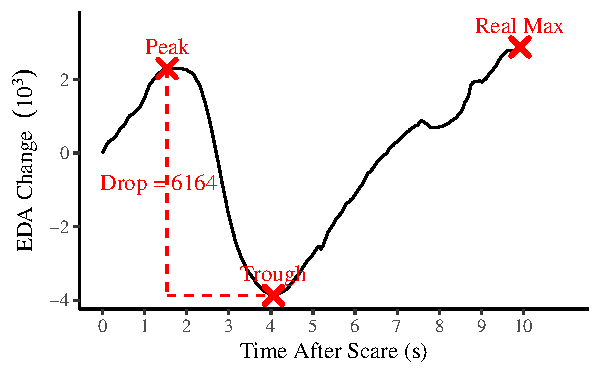
\includegraphics[width=\maxwidth]{figure/ExampleScare-1} 

}



	\caption{How the drop value is calculated}
	\label{fig:ExampleScare}
\end{figure}

The algorithm works as follows:

\begin{enumerate}
	\item 10 seconds after each scare, compute its drop.
	Add it to a list of drops.
	\item If in the calibration phase, return.
	\item Calculate the mean and standard deviation of the drop list, excluding the most recent scare.
	\item Compute the delay factor as in \cref{fig:DelayFactor}, below.
	
	\begin{figure}[H]
  \centering
    \begin{subfigure}[t]{.45\linewidth}
  	\begin{minipage}{\textwidth}
  		\begin{equation}
  		e^{-0.366 * \frac{d - \mu}{\sigma}}
  		\end{equation}
  		
  		where:
  		
  		$d$ is the most recent drop
  		
  		$\mu$ is the mean of previous drops
  		
  		$\sigma$ is the std. dev. of previous drops
  		
  		The delay factor is clamped to values between $\frac{1}{3}$ and $3$, to prevent anomalies causing huge changes.
  	\end{minipage}
  	\caption{Defined Mathematically}
  \end{subfigure}
  \begin{subfigure}[t]{.45\linewidth}
  	\begin{minipage}{\textwidth}


{\centering 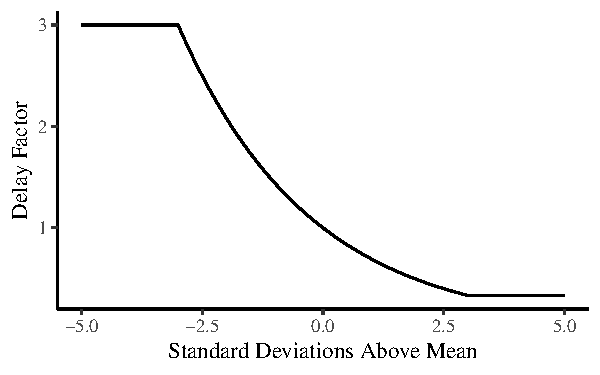
\includegraphics[width=\maxwidth]{figure/DelayFactor-1} 

}



  	\end{minipage}
  	\caption{Visual Representation}
  \end{subfigure}
  \caption{Delay Factor}
  \label{fig:DelayFactor}
\end{figure}
	
	\item Multiply the delay by the factor and clamp it to below 100 seconds.
	\footnote{
		This was done to maintain a sufficiently high scare rate to increase the amount of data available, and might not be necessary if the algorithm was implemented in a real game.
	}.
\end{enumerate}

The delay is not calculated until 10 seconds after the scare.
The delay cannot start to count down until it has been calculated, which results in the real time between scares being between 10 and 110 seconds.

\subsection{Implementation}

\vref{fig:Architecture} shows the hardware and software architecture of the system that was implemented.

An Arduino Uno was used to read from the EDA sensor.
To reduce the noise in the data and to reduce the volume of data recorded, it takes 10 readings and sums them, then reports the sum value.
This still results in frequent data, producing one reading every 5-10 ms.
The Arduino operates in an infinite loop, sending readings to the computer using serial over USB.

\begin{figure}[htb]
	\centering
	\begin{tikzpicture}
	\draw  [thick](-0.5,0.5) rectangle (-3,-0.5);
	\node at (-1.75,0) {Arduino Uno};
	\node (v6) at (-1.75,0.5) {};
	\node at (-1.75,1.5) {EDA Sensor};
	\draw  [thick](-3.5,-1.5) rectangle (0,-5.5);
	\node (v8) at (-3,0) {};
	\node (v7) at (-3.5,-2) {};
	\node (v4) at (-5,0) {};
	\node (v5) at (-5,-2) {};
	\draw  (v4) edge (v5);
	\draw  [->] (v5) edge (v7);
	\draw  (v8) edge (v4);
	\node at (-4,0.25) {USB Cable};
	\draw  (-3.5,-1.5) rectangle (0,-2.5);
	\node at (-1.75,-2) {jrxtx};
	\node at (-1.75,-1.25) {Minecraft};
	\node (v9) at (-1.75,-5) {Delay};
	\node (v10) at (-2.75,-3.5) {Scare};
	\node (v11) at (-0.75,-3.5) {Adjust};
	\node (v12) at (-2.75,-2.5) {};
	\node (v13) at (-0.75,-2.5) {};
	\draw [->] (v10) edge (v12);
	\draw [->] (v13) edge (v11);
	\draw [->] (v11) edge (v9);
	\draw [->] (v9) edge (v10);
	\draw [->] (v10) edge (v11);
	\node at (-4.25,-1.75) {Serial};
	\draw [->] (-1.75,1.5) node (v1) {} circle (0.5);
	\draw [->] (v1) edge (v6);
	\end{tikzpicture}
	\caption{System Architecture}
	\label{fig:Architecture}
\end{figure}

The horror game itself was created as a mod for the game Minecraft.
This meant that the game's implementation was simplified, using Minecraft as a game engine and its mature open-source modding API, forge, to implement custom functionality.
Originally, there was concern surrounding the difficulty of creating a game scary enough that the user's shock would produce a measurable response from the sensor.
However, the sensor is incredibly sensitive.
Even when the user was expecting it, a screen with the word `boo' written on it was enough to get a recognisable response.
This meant that the final jump scare, a scary monster face and loud noise, generated a suitably large effect that could easily be measured and analysed.

The final jump scare is shown in \vref{fig:JumpScare}.
A `creeper' face appears large on the screen, taking up most of the user's field of view.
The creeper is a monster in Minecraft and has a reasonably scary appearance.
At the same time, a loud noise plays \footnote{A video of the jump scare, with sound, is available at \url{https://www.youtube.com/watch?v=kKKoTZelk3k}}.
The noise consists of many in-game noises pitch-shifted and played simultaneously.
It has many low frequencies and some high-pitched scream-like sounds.

\begin{figure}[htb]
	\centering
	
\includegraphics[width=0.5\linewidth]{images/scare.png}
	\caption{The Jump Scare}
	\label{fig:JumpScare}
\end{figure}

The jump scare poses no threat to the player in-game.
Any implementation where the jump scare poses a threat necessarily means that good timing of the jump scare requires environmental knowledge.
The only knowledge used by the algorithm is the timing and effectiveness of previous scares, therefore it must be possible to correctly time the jump scares with only that knowledge, or the algorithm will never time the scares well.

Players were given a task to complete in the game --- to explore a haunted house for 10 minutes, searching for 16 coloured wool in hidden chests.
This goal ensured that participants continued to explore the house throughout their playtest.
The game was set in a haunted house with spooky music playing.
Examples of the game environment can be seen in \vref{fig:GameEnvironment}.
The game environment and music were identical in all playtests, with the environment automatically restored from a backup before each test.
After 10 minutes, the players were automatically informed that the game was complete.
At that point, the jump scares stopped and the data was saved.

\begin{figure}[htb]
	\centering
	\begin{subfigure}[t]{.495\linewidth}
		\centering
		
\includegraphics[width=\textwidth]{images/environment1.png}
	\end{subfigure}
	\begin{subfigure}[t]{.495\linewidth}
		\centering
		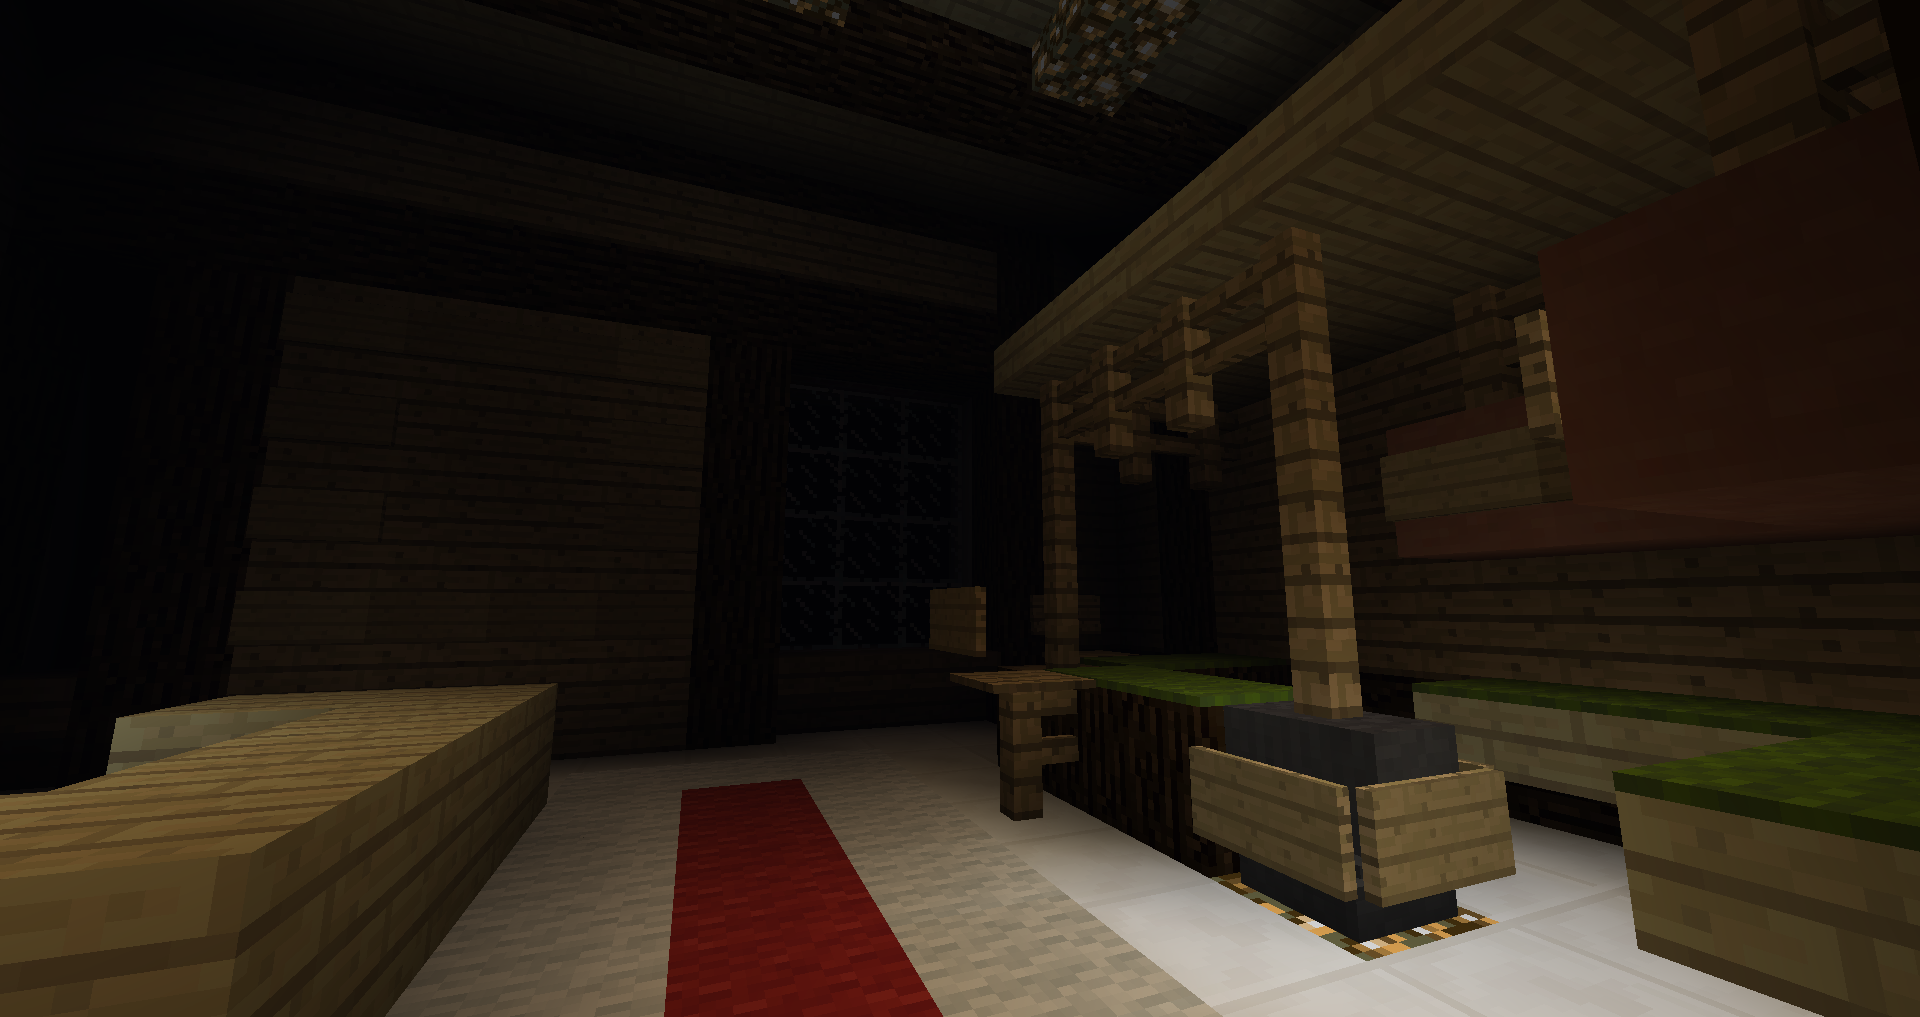
\includegraphics[width=\textwidth]{images/environment2.png}
	\end{subfigure}
	\begin{subfigure}[t]{.495\linewidth}
		\centering
		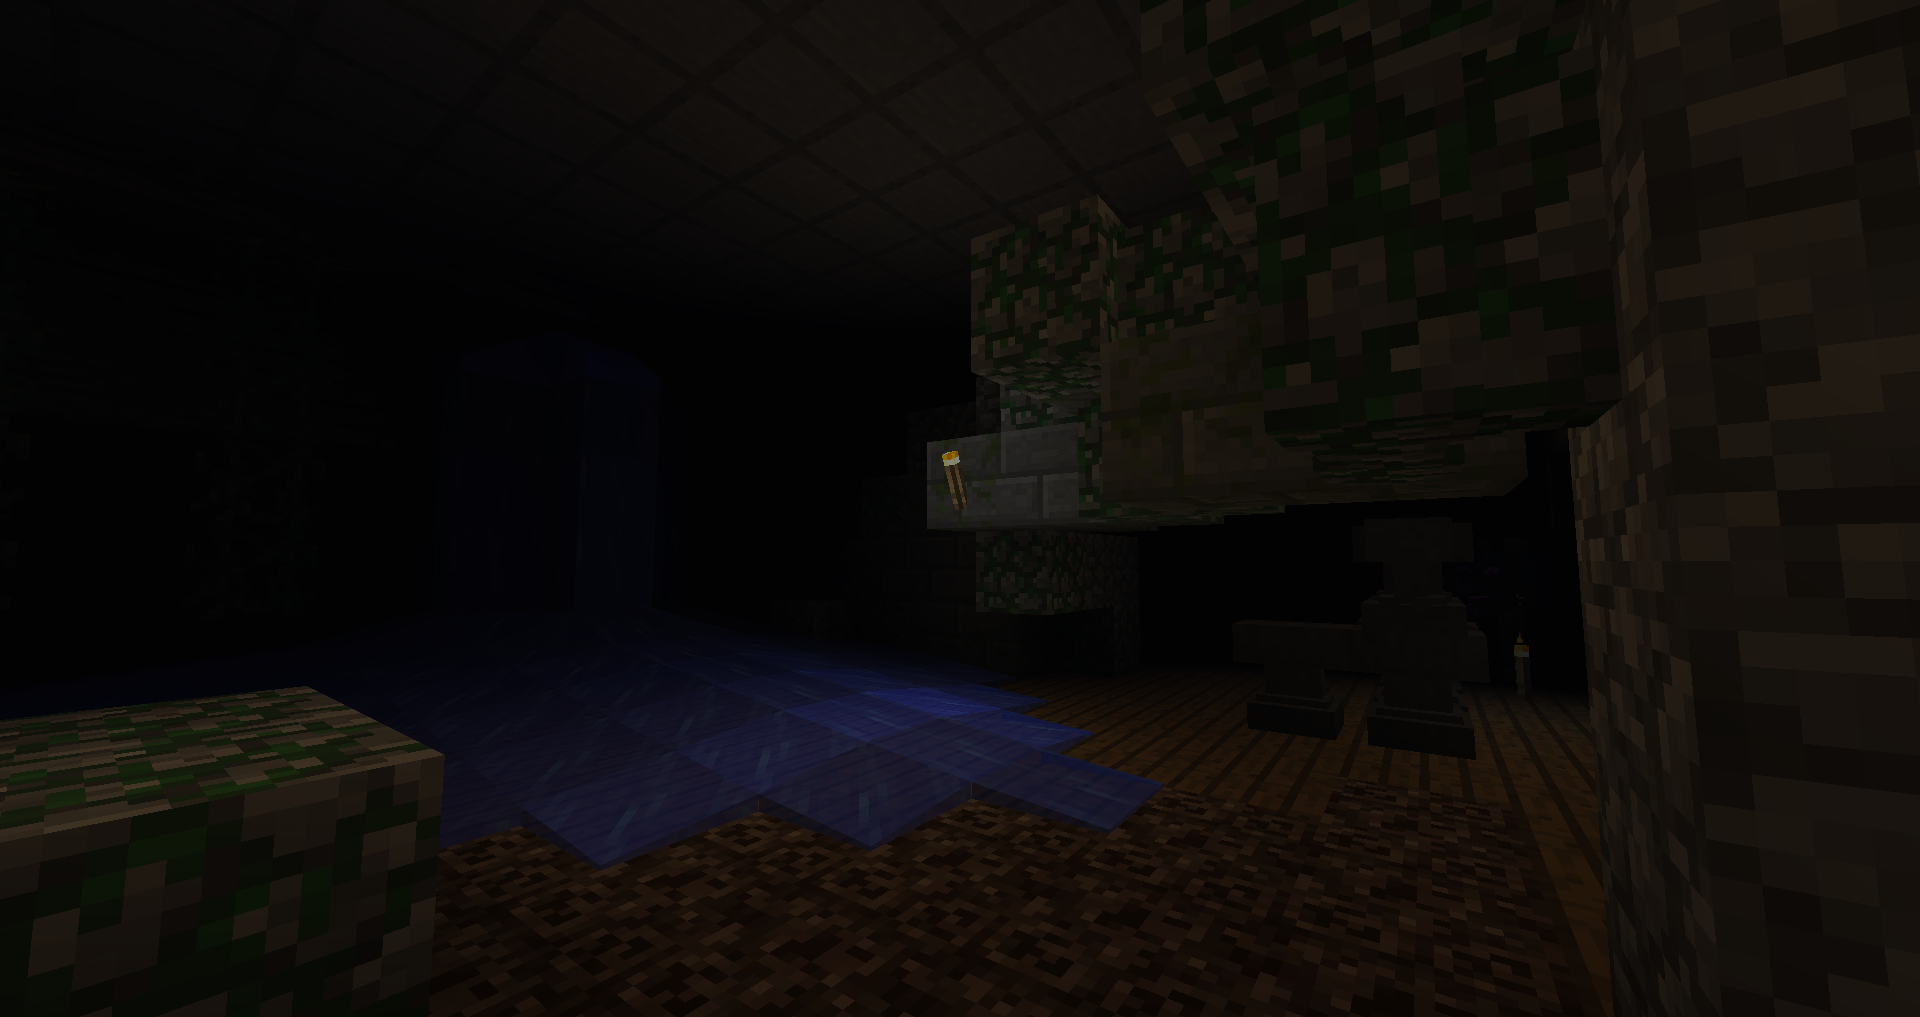
\includegraphics[width=\textwidth]{images/environment3.png}
	\end{subfigure}
	\begin{subfigure}[t]{.495\linewidth}
		\centering
		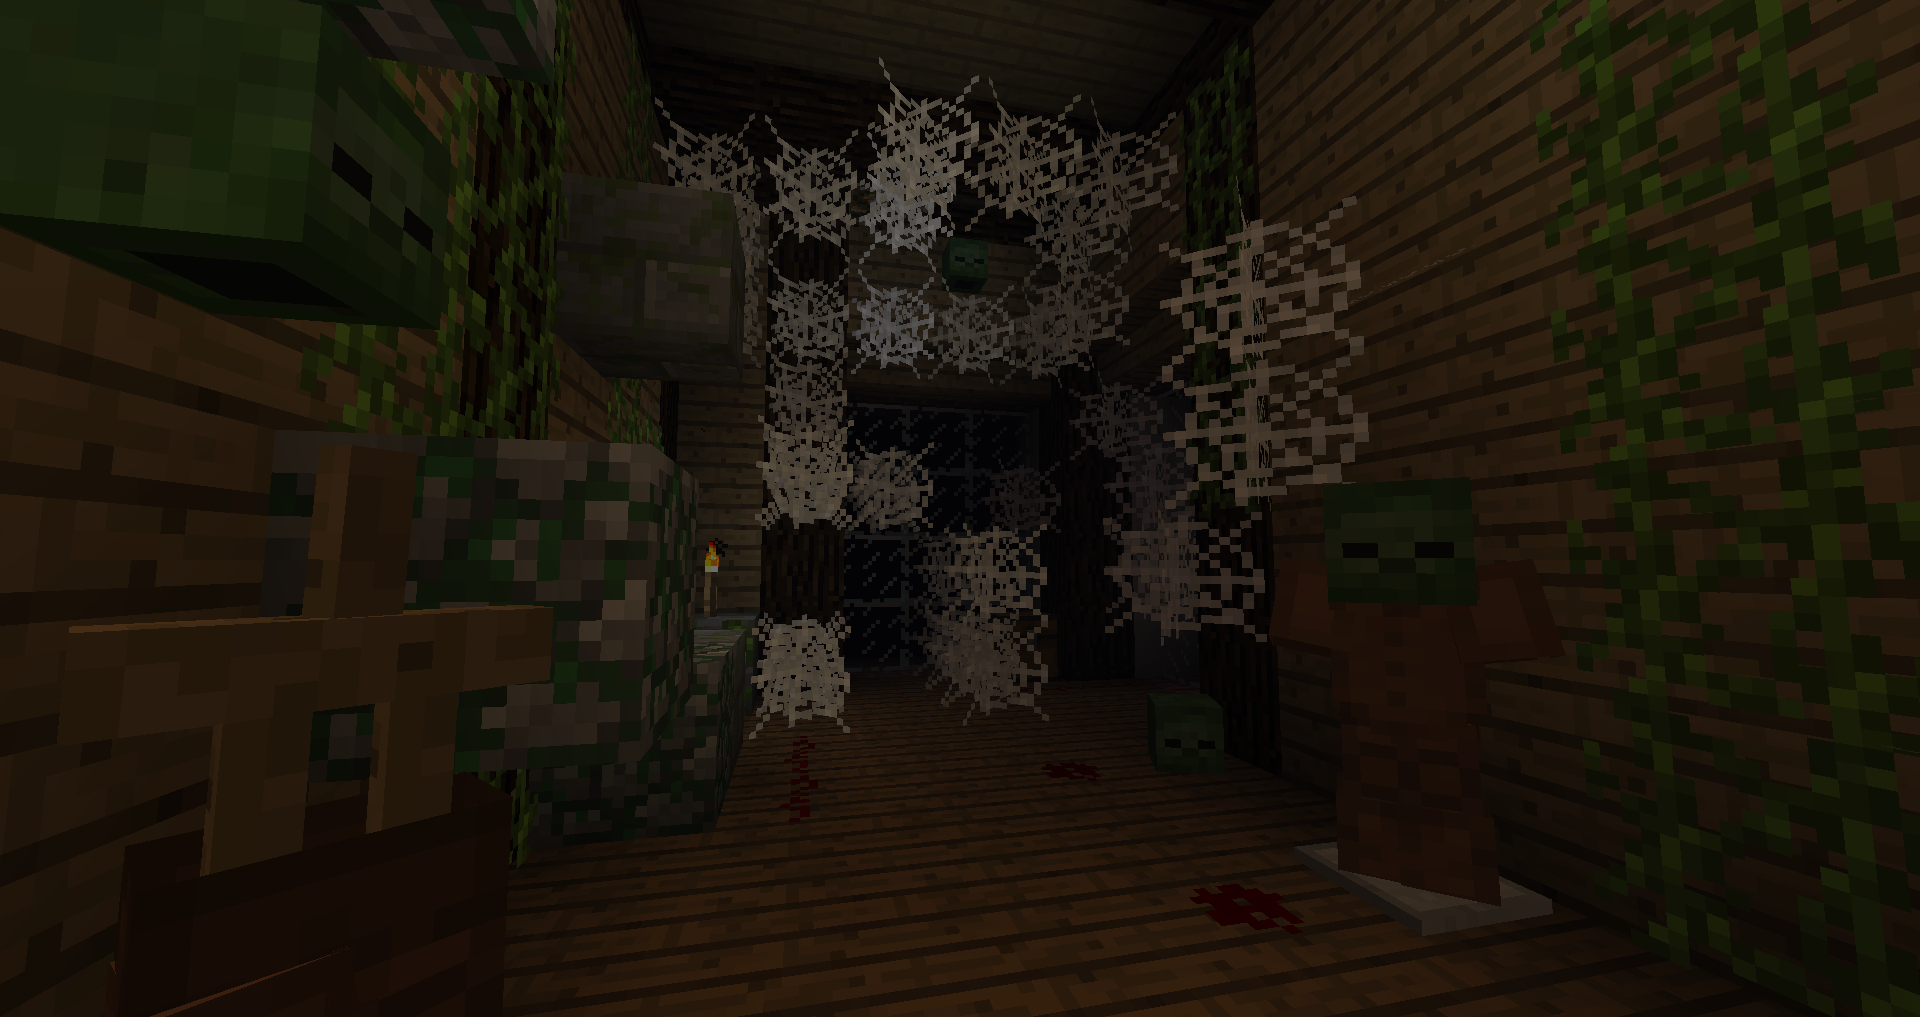
\includegraphics[width=\textwidth]{images/environment4.png}
	\end{subfigure}
	\caption{Examples of the Game Environment}
	\label{fig:GameEnvironment}
\end{figure}


Data from the sensor is recorded for the entire duration of the test, to allow for more flexibility during analysis.
Playtest start and end times are recorded, in addition to the exact timings of the scares.
When the test ends, all data is saved to a JSON file.
These JSON files are used in the `null hypothesis algorithm' for the control group, which simply replicates the scare timings from the data file provided.

\subsection{Software Engineering Design}
Minecraft and Forge are both written in Java, meaning that the choice of language was limited to those able to compile to JVM bytecode.
Of the many options, the language Kotlin was chosen for the system.
The language released in 2011 \cite{kotlinRelease}, and was given first-class support as an Android development language by Google in 2017 \cite{googleKotlin}.
Compared with Java, it is much more expressive and pragmatic, reducing the amount of boilerplate code that must be written to solve a problem.
Kotlin reduces the incidence of common bugs such as null-pointer exceptions by employing nullable types and improving support for functional programming, which was used throughout the system when handling lists and collections.

The Forge modding API abstracts from the real-time nature of a game to an event-based architecture.
The implemented system maintains this style, using an event-based architecture throughout.
Each game tick, which equates to 20 times per second, the API runs the code provided to it.

The Serial code is encapsulated in a separate class.
The Serial code uses the `jrxtx' serial library, which is programmed via pluggable event handlers.
The Serial class attaches its event handler to the library.
This means that every time the library triggers a Serial Event, the Serial class retrieves the serial value and current time, adding them to a large buffer.
The Serial class contains a method to retrieve the last $x$ seconds of data, which is used extensively throughout the rest of the system.

The system is implemented such that it has two interchangeable `storytellers'.
These storytellers filter the game tick events and determine which ones should trigger a jump scare.
There is one storyteller for the tailoring algorithm and one for the null hypothesis algorithm.

The tailoring storyteller maintains a variable which stores the time of the next jump scare and the current delay between scares.
Each tick, it checks whether the current time is after the time stored in the variable.
If so, it triggers the jump scare and nullifies that variable, setting a timer for 10 seconds.
When the timer event triggers, it accesses the last 10 seconds of data from the serial buffer.
Using that data, the delay factor is calculated and the delay updated, in addition to the variable storing the time of the next scare.
From here, the process repeats.

In comparison, the null hypothesis storyteller simply loads a data file outputted during a previous playtest.
The scare times are extracted from the data file and loaded into a queue.
Each tick, the storyteller checks whether the current time is greater than the time at the front of the queue.
If so, it gets dequeued and triggers a scare.
No timer is set since no analysis occurs.

Both storytellers extend from a base storyteller superclass which terminates the playtest after 10 minutes, displaying a `Test Complete' message on the screen.
This triggers the data export, which serialises the data to JSON.

The development of the system followed a mostly waterfall design philosophy, with some agile elements.
Systems that are used in experiments are distinct from most software projects, as the software cannot be changed or updated in any meaningful way once the experiment has began, to preserve the internal validity of the experiment.
Therefore, the system needed to be completed before the experiment began.
However, elements of the agile process were used during the design phase, including repeatedly creating prototype systems and incrementally improving them.
Once the specification for the final system was decided, there was no additional user feedback before the experiment began.
This hybrid approach to software development was the most appropriate for the system, as it allowed flexibility when there were many unknowns, and allowed a fixed system to be used once the experiment began.
A more agile process could have been used, and would have been beneficial, but would have meant running multiple pre-tests, using up participants who could have instead participated in the final experiment.
This would have been ideal, but was infeasible given the limited time and resources available.

In total, the system used for the experiment comprises of 949 lines of code across 21 classes.

\section{Experimental Study}

An experimental study was performed.
The null hypothesis was: `There is no difference between using the algorithm to tailor jump scare timings to the individual player and using a pre-determined set of timings'.
The alternative hypothesis is simply that there is a difference between the groups.

Participants were put into one of two groups:
\begin{itemize}
	\item The intervention group (I-group) played the game with the tailoring algorithm running
	\item The control group (C-group) played the game with jump scare timings pre-determined before they started playing
\end{itemize}

Many controls were put in place in addition to those mentioned in the previous section.

We expect that participants who are more scared of the horror genre will have stronger reactions to the jump scare.
To control for this, each participant was asked to report their general fear of horror films and games.
Participants were then paired such that both participants in the pairing gave the same answer.
One of the participants in the pair was assigned to the I-group, and the other to the C-group.
This is known as `stratified sampling' \citep[p. 178]{stratification}, and means that the distribution in self-reported fear between the two groups is identical, seen in \vref{fig:ParticipantScaredness}.
This stratified sampling controls for participants' self-reported fear, preventing one group from containing more stoic participants than the other, which would have skewed the results.

\begin{figure}[htb]


{\centering 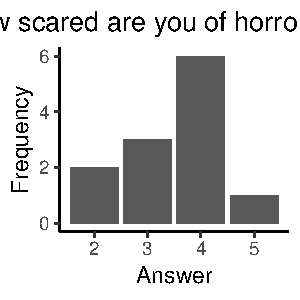
\includegraphics[width=\maxwidth]{figure/ParticipantScaredness-1} 

}



\caption{The distribution of how scared each group is of horror games/films in general}
\label{fig:ParticipantScaredness}
\end{figure}

We expect participants that are shown more jump scares to be more desensitised.
To control for this, each pairing made previously was shown the same number of scares.
Since the scare timing algorithm cannot target a certain number of scares, the I-group participants of each pair were tested first.
When the C-group participants were tested, each person was shown the same number of scares as their partner.
This means that each group has the same distribution of scare frequencies, shown in \vref{fig:ParticipantScares}.

\begin{figure}[htb]


{\centering 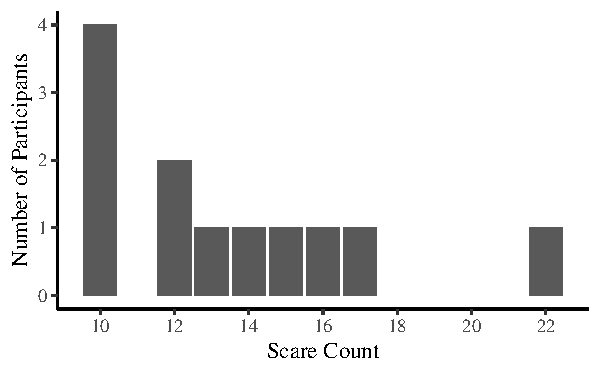
\includegraphics[width=\maxwidth]{figure/ParticipantScares-1} 

}



\caption{Each group's distribution of the number of times a participant was scared}
\label{fig:ParticipantScares}
\end{figure}

The timing of a scare affects the strength of the user's reaction to it.
A number of strategies were considered when creating the null hypothesis algorithm.
Originally, the scares were going to be spread evenly across the playtest, but that meant that participants learned to expect a scare, which unfairly biased the results against the null hypothesis algorithm.
This belies that a set of scare timings have an inherent `quality' to them, unrelated to whether the scares were tailored to an individual.
To ensure that this underlying `quality' of timing was the same between the two groups, each C-group participant was scared at the exact same times as their I-group partner.
This means that the timings were based on the participant's partner's response to the scare, not theirs.

A discussion of the experiment's issues, and the threats to its validity, can be found in \hyperref[sec:Validity]{\cref{sec:Evaluation}, \vref{sec:Validity}}.

The study originally aimed to test 50 participants.
Due to practical issues, only 26 participants were tested.
Of those, 2 participants were excluded from analysis as their EDA went below zero and the sensor stopped working, corrupting the data.
Of the remaining 24 participants, 12 were allocated to each group.
After 21 participants, Easter break was arriving and people would start to leave Durham, meaning that finding additional participants would become impossible.
At that point participation was limited to those who could complete a pair that only had its I-group participant.
Prospective participants were not told what answer was needed on the self-reported fear question.

\subsection{Ethics}
Participants signed an informed consent form which explained what the study entailed and the experimental setting.
Harm was prevented by allowing participants to ask questions, see the jump scare, and drop out freely.
Confidentiality was achieved by using participant IDs and only linking ID to name in the consent forms, which were securely destroyed after the experiment was complete.
Data was stored on a password-protected device and only published if the participants signed the voluntary data release.
The voluntary data release was signed by all participants, and as such the raw data has been released into the public domain.
Previous research has not covered this topic, meaning that the outcome of the experiment was uncertain, and there were no ethical concerns surrounding wasting participant time to confirm an already known outcome.

\section{Results}

First we will examine the results of the questions asked to participants after their playtest was completed, before moving on to analyse the raw data from the sensor.

Participants were asked how much they enjoyed their time playing the game.
The answers given by each group are presented in \vref{fig:ParticipantEnjoyment}.
In general, participants in the intervention group enjoyed the game less than those in the control group.

\begin{figure}[htb]
  \centering
  \begin{subfigure}[t]{.49\linewidth}


{\centering 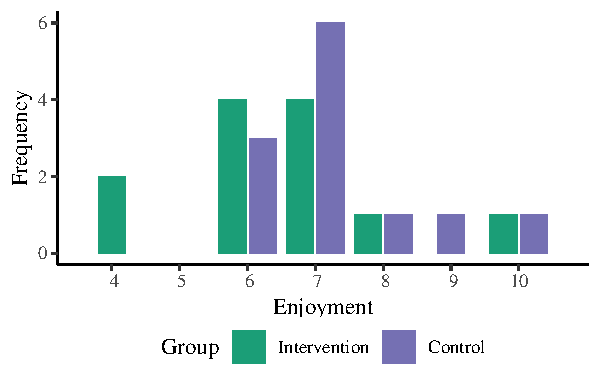
\includegraphics[width=\maxwidth]{figure/ParticipantEnjoyment-1} 

}



  	\caption{Distribution of Responses}
  \end{subfigure}
  \begin{subfigure}[t]{.49\linewidth}


{\centering 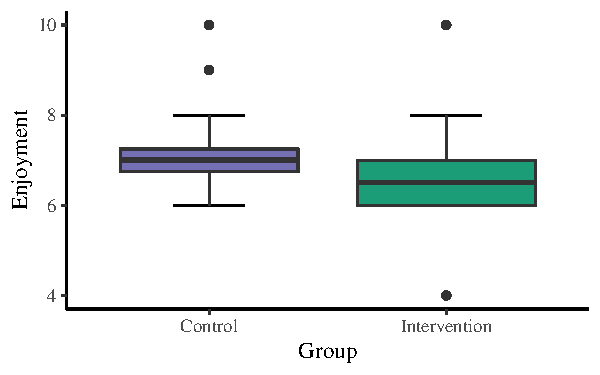
\includegraphics[width=\maxwidth]{figure/ParticipantEnjoymentBoxPlot-1} 

}



  	\caption{Comparison between Groups}
  \end{subfigure}
  \caption{On a scale of 1-10, how much did you enjoy that as a game?}
  \label{fig:ParticipantEnjoyment}
\end{figure}

Participants were asked to rate the frequency of the jump scares from "Far Too Few" to "Far Too Many" jump scares.
The answers given by each group are presented in \vref{fig:ParticipantTiming}.
Most participants felt there were too many jump scares.
Their feeling is backed up by the scare timing histogram in \vref{fig:ScareHistogram}.
Generally, the algorithm decreased the frequency of jump scares over time.

The control group felt marginally more strongly that there were too many scares.
Since the two groups had identical scare timings, this was not the result of any difference in the real frequency between the groups.
Therefore, this suggests that the scares were badly timed for the control group, making them more aware of the scares and making the scares less immersive.

Graph B in \cref{fig:ParticipantTiming} shows a statistically significant correlation between the real frequency of scares and the participants' perceived scare frequency.
This indicates that participants are accurately assessing the frequency of jump scares and that we are not just seeing trends in random data.

\begin{figure}[htb]
  \centering
  \begin{subfigure}[t]{.49\linewidth}


{\centering 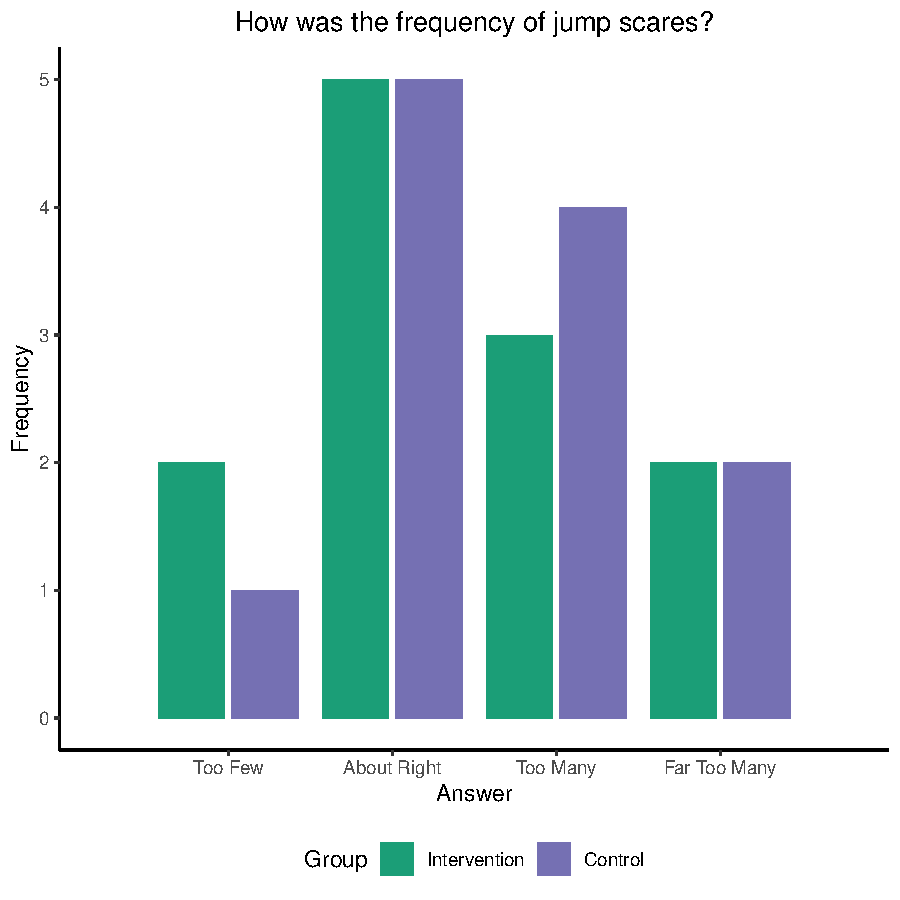
\includegraphics[width=\maxwidth]{figure/ParticipantTiming-1} 

}



		\caption{Distribution of Responses}
  \end{subfigure}
  \begin{subfigure}[t]{.49\linewidth}


{\centering 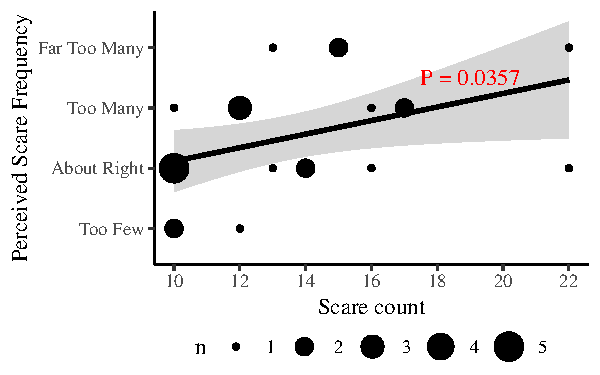
\includegraphics[width=\maxwidth]{figure/ScareFrequency-1} 

}



  	\caption{Actual vs Perceived frequency}
  \end{subfigure}
  \caption{How was the frequency of jump scares?}
  \label{fig:ParticipantTiming}
\end{figure}

\begin{figure}[htb]


{\centering 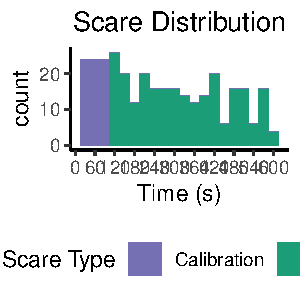
\includegraphics[width=\maxwidth]{figure/ScareHistogram-1} 

}



\caption{Scare Frequency over Time}
\label{fig:ScareHistogram}
\end{figure}

We will now discuss the data recorded from the EDA sensor.
The raw data from the sensor is shown in \vref{fig:RawData}.
This has already been normalised so that the playtest starts at $x=0$.
The actual data records wallclock time for each measurement as well as wallclock time for when the playtest starts, which we used to normalise the data.

This data requires significant cleanup before it is ready to be analysed.
The data was recorded in full so that the relevant parts could be extracted during analysis --- so as to not make any analysis decisions pre-emptively.

The drop is calculated using the 10 seconds after each scare.
\vref{fig:PerGroupScares} shows the data after filtering to just the 10 seconds after each scare and colouring the lines based on which group the participant is in.
Lines with a larger vertical drop generally indicate a person that was more scared by the jump scare.

\begin{figure}[htb]
	\centering
	\begin{subfigure}[t]{.49\linewidth}


{\centering 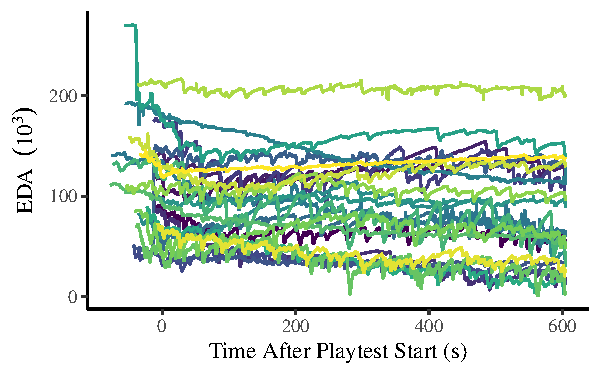
\includegraphics[width=\maxwidth]{figure/RawData-1} 

}



		\caption{Raw data from the sensor}
		\label{fig:RawData}
	\end{subfigure}
	\begin{subfigure}[t]{.49\linewidth}


{\centering 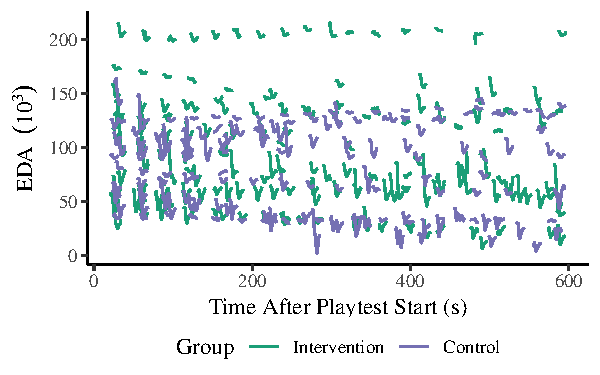
\includegraphics[width=\maxwidth]{figure/PerGroupScares-1} 

}



		\caption{Scare data, coloured per group}
		\label{fig:PerGroupScares}
	\end{subfigure}
	\caption{Data pre-analysis}
	\label{fig:Data}
\end{figure}

By normalising all of these scares to start at $x,y = 0$, and taking the mean of each group's lines, we can see each group's average scare.
We can also calculate a standard error margin around these means.
When doing this, we filter out the first 3 scares for each participant as the algorithm hasn't kicked in so they're essentially both control groups.
\vref{fig:ResponseAfterScare} shows the average scare for each group and the difference between the two groups.
The two groups are significantly different, with participants in the intervention group seeing their EDA fall for longer and to a lower trough value.
The intervention group also takes longer to recover, with the two lines still being separated by more than the margin of error after 10 seconds.
Additionally, the intervention group reacts slightly quicker than the control group, with the EDA starting to drop slightly earlier than it does for the control group.

\begin{figure}[htb]
  \centering
  \begin{subfigure}[t]{.49\linewidth}


{\centering 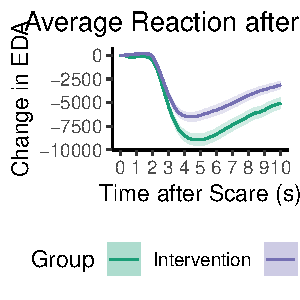
\includegraphics[width=\maxwidth]{figure/ResponseAfterScare-1} 

}



    \caption{Per-Group Average}
  \end{subfigure}
  \begin{subfigure}[t]{.49\linewidth}


{\centering 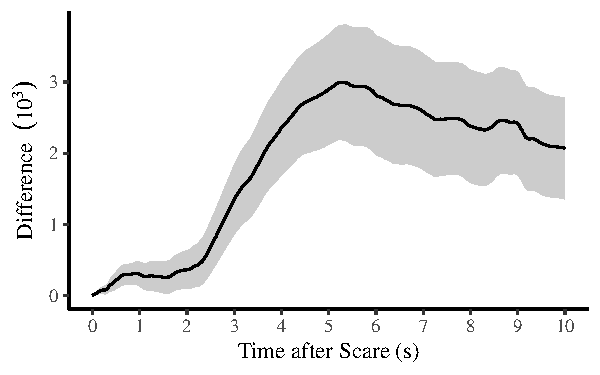
\includegraphics[width=\maxwidth]{figure/CompareGroups-1} 

}



    \caption{Difference between Groups}
  \end{subfigure}
  \caption{Average Response to a Jump Scare}
  \label{fig:ResponseAfterScare}
\end{figure}

\begin{figure}[htb]
	\centering
	\begin{subfigure}[t]{.49\linewidth}


{\centering 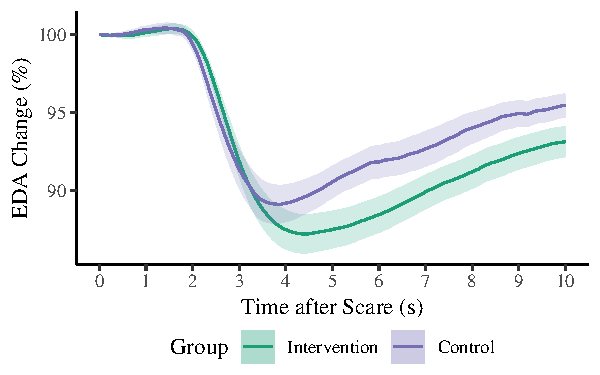
\includegraphics[width=\maxwidth]{figure/ResponseAfterScareRel-1} 

}



		\caption{Per-Group Average}
	\end{subfigure}
	\begin{subfigure}[t]{.49\linewidth}


{\centering 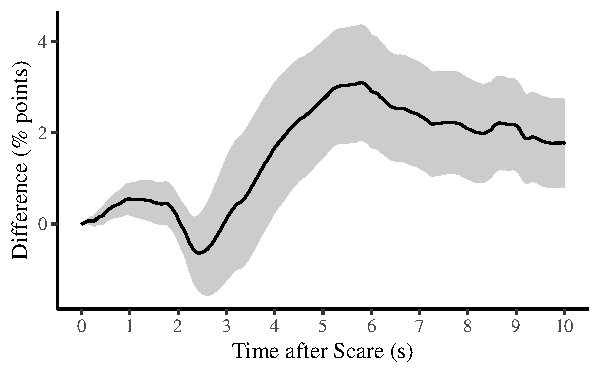
\includegraphics[width=\maxwidth]{figure/CompareGroupsRel-1} 

}



		\caption{Difference between Groups}
	\end{subfigure}
	\caption{Average Relative Response to a Jump-Scare}
	\label{fig:ResponseAfterScareRel}
\end{figure}

If we take the data from \vref{fig:PerGroupScares}, and convert each scare line to its calculated drop value, we can plot how the size of the drop changes over time.
\vref{fig:ScarednessOverTime} shows every scare that occurred during the experiments, and plots one linear regression per group.
At the time of the first scares, the linear regressions predict almost exactly the same scaredness between the two groups.
This is a strong indication that the sample is valid and that the two groups begin with the same reactions before the algorithm has kicked in.
As time goes on, the linear regressions diverge, separating by more than a 95\% confidence interval by the mid-way point of the playtest.
This indicates that the timing algorithm prevents the intervention group from becoming bored by the jump scares, while the control group does become bored without it.

\vref{tab:RegressionTable} shows the relevant statistics of the two regressions.
The P-Value of the control group is under 0.01, and its gradient is negative, indicating a statistically significant trend.
Over time, the control group becomes less scared of the jump scares.
The R-Squared value indicates that around 4\% of a control-group participant's response to a scare can be predicted solely by how long they have been playing.
The gradient indicates that for each second played, a participant in the control group would respond to a scare with a drop that is 8.5 points smaller.

In comparison, the P-Value of the intervention group is above 50\%, indicating that it's likely there is no correlation between time played and scaredness in the intervention group.
Even if there was a correlation, the gradient is positive indicating that participants actually become more scared over time.

\begin{figure}[htb]
  \centering
  \begin{subfigure}[t]{.49\linewidth}


{\centering 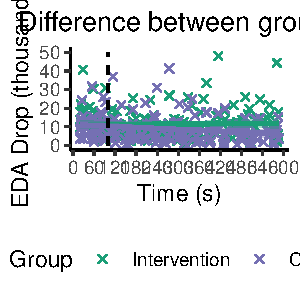
\includegraphics[width=\maxwidth]{figure/ScarednessOverTime-1} 

}



    \caption{All data}
  \end{subfigure}
  \begin{subfigure}[t]{.49\linewidth}


{\centering 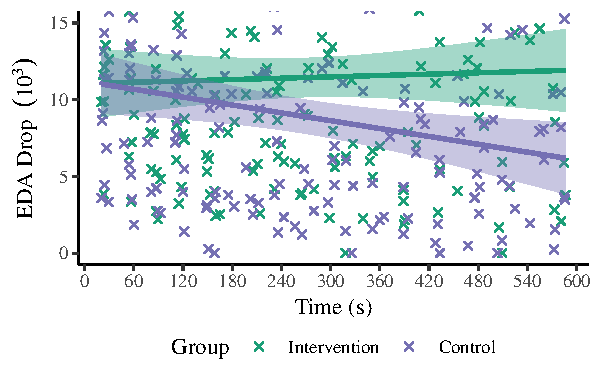
\includegraphics[width=\maxwidth]{figure/ScarednessOverTimeCrop-1} 

}



    \caption{Cropped}
  \end{subfigure}
  \caption{Scaredness over Time}
  \label{fig:ScarednessOverTime}
\end{figure}

\begin{table}[t]

\caption{\label{tab:RegressionTable}Relevant statistics for the Regressions}
\centering
\begin{tabular}{cccc}
\toprule
\textbf{Model} & \textbf{Gradient} & \textbf{R-Squared} & \textbf{P-Value}\\
\midrule
Intervention & 1.47 & 0.001 & 0.695\\
Control & -8.54 & 0.042 & 0.009\\
\bottomrule
\end{tabular}
\end{table}


\section{Evaluation}
\label{sec:Evaluation}
\subsection{Threats to Validity}
\label{sec:Validity}
The threats to the validity of the study will be analysed using the framework described in \citet[pp. 5--6]{validity}.

\subsubsection{Internal Validity}
The internal validity concerns whether the experiment is successfully measuring the effect that it tries to measure. Some factors affecting interval validity will be discussed:

\textbf{Maturation} --- When the measured variable is a function of time and there is a difference in time between the testing of the two groups.
Since in each pair the intervention group participant is tested first, the intervention group tests on average happened before the control group tests.
However, it is unlikely that the dependent variable is a function of time - people are not any more or less scared of horror games from one week to the next and there were no newsworthy events that could have heightened people's sense of fear.

\textbf{Testing} --- When participants take multiple tests and the first test affects future tests.
This would have been a serious issue, but was controlled for by having each participant only do a playtest once.

\textbf{Instrumentation} --- When the sensor/observer changes and produces different results.
This was not an issue, as the sensor and observer was consistent throughout the experiment.
The experiment was only single-blind, but as most data was recorded automatically it was not affected by the observer knowing the participant's group.

\textbf{Attrition} --- When the risk of people dropping out / being excluded is a function of the dependent variable.
This risk is present in two ways.
If people are very scared, their EDA will drop more (dependent variable), and those people will also be more likely to drop out.
Therefore if one group is much scarier the result won't show as clearly as some will drop out over being too scared.
This risk had no impact as nobody dropped out once starting the playtest.
%TODO
Two participants were excluded because their skin resistance was so low that the sensor broke.
At first, this appears like a serious attrition risk.
However, the low skin resistance was not due to a large drop, but due to their naturally low baseline skin resistance.
This means that the attrition was caused by factors unrelated to the experiment.
Therefore, attrition threats are minimal.

\textbf{Selection of Subjects} - When the two groups are not comparable.
Much of this was controlled for using stratification during sampling.
However, the I-group and C-group participants likely differed, since the participants were assigned to groups chronologically.
Since the I-group participants were in general found earlier than the C-group participants, the I-group participants will be closer friends with the researcher, as participants were naturally selected based on availability.
This threat could be reduced by sampling participants randomly, getting an initial expression of interest and a self-reported fear rating, then assigning groups and performing tests.
This was planned originally, but found to be infeasible due to the increased attrition rates of having a two-phase sampling strategy.

Additionally, participants begin the playtest with different EDA levels.
As higher EDA leads to larger drops as a result of the same stimulus, this makes it harder to compare between the groups.
There is a difference in starting EDA between the groups, seen in \vref{fig:StartingEda}.

\begin{figure}[htb]


{\centering 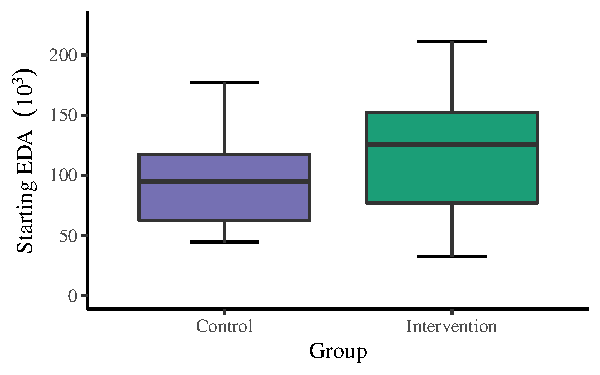
\includegraphics[width=\maxwidth]{figure/StartingEda-1} 

}



	\caption{The starting EDA for each group}
	\label{fig:StartingEda}
\end{figure}

	
\textbf{Environmental} - When the test environment changes differs between participants.
Some tests were performed in a university computer science department, which contains many distractions, while other tests were performed in quiet, private areas.
Additionally, some tests were performed at social events, meaning that participants had been drinking alcohol - though no participant was noticeably drunk.
These factors were not recorded and therefore it is impossible to investigate any correlation between the environmental/demographic factors and results.

\textbf{Data Vandalism} - When the data is intentionally corrupted by the participants.
There is a slim chance of intentional data vandalism.
Participants could lie about how scared they were, but if we plot a scatter graph as in \vref{fig:ReportedScaredness}, we don't see any clear evidence of lying.
People generally follow the regression line, but with a wide variance.
A few clear anomalies could indicate data vandalism, but this wide variance instead suggests that people are inaccurate when judging their fear.
Participants could train themselves to change their EDA at will, usually done to beat a lie-detector test.
That would be hard to detect, by design, but nobody showed any prior knowledge of EDA or GSR.
It's hard to rule this out but it's a very niche skill and the chance of someone having that skill and intentionally vandalising the data is negligible.

\begin{figure}[htb]


{\centering 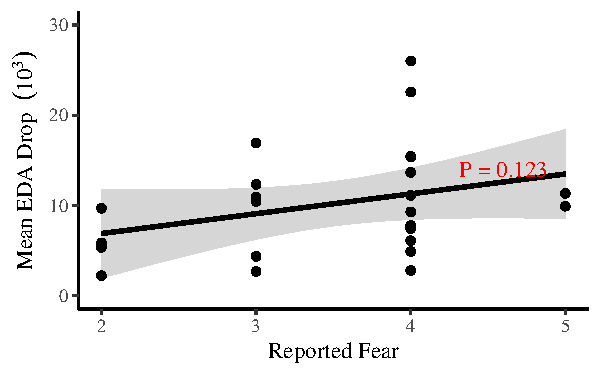
\includegraphics[width=\maxwidth]{figure/ReportedScaredness-1} 

}



	\caption{Drop size positively correlates with reported scaredness}
	\label{fig:ReportedScaredness}
\end{figure}

\subsubsection{External Validity}
The external validity concerns whether the experiment is generalisable to the population.
Two factors impacted the external validity.

\textbf{Interaction effects of selection biases and the experimental variable} - When the sample is not representative of the population and reacts differently.
The majority of participants were young, male, and many of them were computer scientists.
It is not clear whether these participants would react to the intervention differently than the population.
Therefore, it is impossible to rule out this threat.

\textbf{Not generalisable to realistic gameplay} - When the experimental arrangements are different to the real-world use of the intervention.
It is not clear whether a 10-minute test would generalise to a multi-hour play session, but limiting the test length was necessary for practical reasons.
Additionally, it's not clear whether a simple game based in Minecraft where all jump scares are the same would generalise to a more complex game, with multiple kinds of jump scare.
Limiting the test to a simple game was necessary in this first experiment to control for as many factors as possible, but means that additional tests with more complex games will be necessary before we can be confident that the data is generalisable to real-world use.

\subsection{Analysis}
%TODO reword from here
There is a slight difference in participant enjoyment between groups, as seen in \vref{fig:ParticipantEnjoyment}.
Since it's a small difference, it could just be random due to the small sample size.
Or it could be due to biases in the sampling as discussed earlier.
Additionally, only one question about enjoyment was asked in the post-test questionnaire, and no demographic data was recorded, so we can't drill down to look into what could be causing a difference between groups.
Finally, the participants aren't the target audience for a horror game, as enjoying horror games wasn't a requirement to take part.
Further study to explore whether the algorithm improves enjoyment in horror-game players would be warranted.
It seems suspect that a horror game (that's not very scary to begin with) can become more scary but less enjoyable just by changing the timings.
Intuitively, those should be correlated.
This runs counter to intuition, which means it would be interesting to study further, but it's a small difference in a study with a small sample size, so it could easily just be random chance.
The use of a 10-point scale increases the effect of randomness.

There's a very marginal difference between groups when it comes to the perceived frequency of jump scares, as seen in \vref{fig:ParticipantTiming}.
It's fairly reassuring that the groups are so similar, seeing as they had the exact same timings, and that's what they were supposed to be rating.
This could be interesting to investigate further, and with a larger sample size you could say conclusively that there is a difference between groups.
If there is a difference between groups, this could be the beginning of further research into the perceived frequency of jump scares based on good vs bad timing.
As a purely theoretical excercise about the perception of horror games, there would be no requirement to use an algorithm.
You could just have a person manually trigger the jump scares at good times.
Would be interesting to control the number of jump scares but not the timing, then compare good vs bad timing and see how people rate the scare frequency.

\vref{fig:ScareHistogram} shows that the algorithm decreased the number of scares over time.
This suggests that the initial scare frequency was too high.
The intial scare frequency has a scare happening every 20-30 seconds, meaning 20-30 scares over the 10-minute playthrough.
This number was chosen to get the calibration tests over with quickly to maximise the amount of test data (since the first 3 scares are just for calibration and the algorithm hasn't kicked in).
However, participants found 20-30 scares in a playtest far too high.
Figure (b) in \cref{fig:ParticipantTiming} shows that around 10 scares is the ideal number.
Changing the starting frequency to around 1 scare per minute would result in a more ideal number of scares.
This would intuitively make the game more immersive and scarier.
That's not really necessary - the sensor is sufficiently sensitive to detect small changes.
Therefore the benefit of more data outweighs the downside of having a less scary game due to having too many scares.
A more well-funded study could perform longer tests with a more appropriate scare frequency and get slightly better data.
I don't think the high scare frequency invalidates any of the data.

\vref{fig:ResponseAfterScare} is one of the more significant outcomes of the project.
The intervention group is significantly more scared than the control group.
They drop further, faster, and for longer.
However, the intervention group also starts at a higher EDA, so their drops will naturally be bigger.
The intervention group also does not recover faster.
Due to the mechanics of EDA, a shock produces sweat which takes time to evaporate before the EDA can recover.
The fact that the intervention and control groups recover at almost the same speed lends itself to the validity of the data, as opposed to an error in the measurement.
I think the intervention group probably was more scared than the control group.
A bigger study with many more participants would be far better at judging this - as they could get a better sample and control for starting EDA.

In \vref{fig:ResponseAfterScareRel}, we look at the relative drop instead.
This completely removes the effect of higher EDA having larger drops.
However, this actually biases the data in the other direction.
Interestingly, the two lines now drop at around the same time, and drop at roughly the same speed.
However, the intervention group line drops for longer and to a lower trough value.
The two lines end up more than a margin of error apart.
This indicates that the starting EDA is not the reason for the difference between the groups.
It is likely that the intervention causes the intervention group to be more scared by the jump scares.
It would be good to conduct more research and ask the participants how scared they felt, to see whether the feeling is directly correlated to EDA, or whether there are other aspects that have not been captured in our model.

\vref{fig:ScarednessOverTime} is one of the most convincing pieces of evidence for the success of the intervention.
The two groups have almost identical reactions to the first jump scares, before the algorithm starts.
In the control group, there's a strong downwards trend over time, with participants becoming bored of the jump scares and not reacting nearly as much.
Meanwhile, in the intervention group there is no such trend.
More importantly, since we are not comparing the groups to each other but to themselves at an earlier time, the issues of different starting eda between groups is not relevant.
Although a longer test would be needed to confirm it, this chart strongly suggests that the algorithm will improve the longevity of a horror game, and allow players to play for longer before becoming desensitised to the scares.

\section{Conclusions}

This project implemented an algorithm which controlled the timing of jump scares based on data from an EDA sensor attached to the player.
The algorithm increased scare frequency when the player had an above-average reaction, and decreased scare frequency when the player had a below-average reaction.
The `average reaction' is determined per-participant, using a 3-scare calibration period at the start of a playtest.

Almost all deliverables were successfully completed.
All minimum deliverables were completed --- a hanted house environment was created for players to explore, and their EDA was tracked while doing so.
The jump scare was created based on preliminary user testing, and due to the high sensitivity of the sensor, could be made less scary than otherwise necessary, making the game more accessibly to players who rarely engage with the horror genre.
Data from users is continuously analysed and future scares are timed based on delay since previous scares and the effectiveness of previous scares.
A null hypothesis algorithm was created which scared users on the same schedule as a previous player, as opposed to algorithmically tailoring the timings to the player.
A user study was conducted, which will be discussed in great detail below.
The algorithm was not revised based on the user study due to lack of time and infeasibility of gathering a second sample of users who had not already played the game.

The user study compared an intervention group, who played with the algorithm enabled, and a control group, who played with pre-determined timings.
The study controlled for self-reported fear of horror games, scare frequency, and scare timing.
The scare timings for the control group were determined by copying the timings for a member of the intervention group that reported the same level of general fear.
This means that the intervention group and control group had the same timings, just that the timings were tailored for the intervention group and not the control group.
The main weaknesses of this study were the small sample size ($n=24$) and that initial EDA was not controlled for.
Initial EDA was significantly higher in the intervention group, which means that the same scaredness would cause a larger absolute drop in EDA and a smaller relative drop in EDA.

The intervention group reported that the game was slightly less enjoyable and that scares were marginally less frequent compared to the control group.
The small sample size and small effect size mean that no conclusions can be made about the intervention's effect on enjoyableness or perceived scare frequency.

The intervention group had a larger reaction on average, whether looking at the absolute or relative change in EDA.
By both measures, the two groups were more than the margin of error apart, strongly suggesting that the algorithm is effective in making players more scared.
The fact that both absolute and relative drops were bigger suggests that this is not simply due to the difference in initial EDA.

The intervention group's scaredness did not decrease over time ($P = 0.695$).
The control group's scaredness decreased over time ($P = 0.00938$).
Since we are comparing each group to itself at an earlier time, initial EDA has no effect.
We can conclude the the algorithm was successful at preventing players from becoming desensitised to the scares.

The validity of these two results is questionable, due to a number of environmental factors that were not controlled for.
The user study was conducted across multiple locations, and some participants had been drinking alcohol, though none were noticeably drunk.
Some environments were more distracting than others, and the distractions can cause changes in EDA.
As a side effect of controlling for particpants' self-reported fear, the participants were not assigned to groups randomly but instead chronologically.

I would recommend further research into this algorithm and the use of EDA for tailoring horror games, as this study provides promising preliminary results.
Future research should conduct all tests in a controlled environment without distractions.
Additionally, a larger sample size should be gathered, which will help to get a more equal distribution of initial EDA between groups.
When gathering the sample, participants should be asked to register interest and self-report their fear of horror games, before being randomly assigned to groups.
This would probably require some incentive to participate to reduce participant attrition after the initial expression of interest.
Additionally, the research should explore if the algorithm prevents desensitisation over longer periods, as this study only tested each participant for 10 minutes.
Showing this would be necessary to recommend incorporating the algorithm into commercial games, as players can play for hours at a time and expect the game to remain scary throughout.

Future avenues for research could involve using additional sensors, such as a heart rate sensor.
This would allow the system to sense tension in the user, which could be incorporated into a more complex algorithm which tries to scare users when they are feeling most tense.
Alternatively, future research could extend the algorithm to use multiple kinds of scares, finding out which kind of scare is most effective for a given participant.
For example, a person with arachnophobia would have a larger response to spider-based scares so the system would see that and include more of them.

This study shows promising results but does not provide enough convincing evidence for me to recommend incorporating the algorithm into commercial games at this time.
There are too many threats to the validity of the study to be confident that the results are correct, and there is little evidence that the results are generalisable to more complex games with longer play times.
With confirmation from further study that is more well-funded and with fewer threats to its validity, this algorithm could be incorporated into horror games.
If successfully integrated into a commercial game, this algorithm shows great promise for both developers and players.
For developers, they would no longer need to manually program where each scare should go, as it would automatically be tailored to the player.
For players, they would get to enjoy a scarier game, and would be able to play the game multiple times through without learning where the scares are and expecting them, massively improving replayability.


\section{References}
\footnotesize\bibliography{projectpaper}
\end{document}
